%%%%%%%%%%%%%%%%%%%%%%%%%%%%%%%%%%%%%%%%%%%%%%%%%
%
%     Chapter 2
%
%%%%%%%%%%%%%%%%%%%%%%%%%%%%%%%%%%%%%%%%%%%%%%%%

\chapter{Background}
\label{two}

\section{SIMD and SWAR}
SIMD is a parallel computing concept that performs the same instruction on different data to exploit data parallelism. Most of today's commodity processors supports SIMD within a register (SWAR). In this model, SIMD operations are applied within general-purpose or special registers that may be considered to be partitioned into fields. Operations on each field are independent from each other. This means for example, carry bits generated by addition could not pass to the next field.

The other important feature of the SWAR model is that the partition is not physical but rather a logical view of the register, so that different views are available on the same register. For a 128-bit SIMD register, a valid partition can be sixteen 8-bit fields as well as four 32-bit fields. There is no penalty from switching the logical view.

Some popular SIMD instructions sets are listed here:
\begin{itemize}
  \item Intel MultiMedia eXtension (MMX). It defines eight 64-bit registers known as MM0 to MM7 which are aliases of the existing IA-32 Floating-Point Unit (FPU) stack registers. MMX only provides integer operations for early graphical applications thus is not a general purpose instruction set for SIMD programming \cite{hua_idisa}.

  \item Intel Streaming SIMD Extensions (SSE) series. SSE extends the MMX instructions set and it introduces eight new independent 128-bit SIMD registers known as XMM0 to XMM7. Its successor SSE2 adds a rich set of integer instructions to the 128-bit XMM registers which makes it a useful SIMD programming model. AMD added support for SSE2 in its AMD64 architecture soon after the Intel released SSE2, making SSE2 broadly available across the desktop computers. Intel then released SSE3, SSSE3, SSE4 and AMD released SSE4a as the following SSE generations.

  \item Intel Advanced Vector Extensions (AVX). AVX extends the size of SIMD registers from 128 bits to 256 bits. It introduces 16 new registers YMM0 to YMM15 but still supports the 128-bit SSE instructions. More importantly, AVX shifts the two-operand operations towards the non-destructive three-operand form. Three-operand operation preserves the content in operand registers and could reduce the potential movement of data between registers. AVX supports a number of floating point operations on 256-bit registers, but does not support many of the integer operations that exist in SSE\@. Its successor AVX2 fills this gap and ensures the transition from SSE to AVX instructions with the same programming model. AVX2 is available on the Intel Haswell architecture. Its successor AVX512 has been announced to support 512-bit SIMD registers.

  \item ARM NEON\@. ARM as a popular mobile platform introduces its own SIMD extension named NEON in their Cortex-A series processors. It has thirty-two 64-bit registers (D0 to D31) as well as sixteen 128-bit registers (Q0 to Q15). In fact, $\text{D}_{2 \times i}$ and $\text{D}_{2 \times i + 1}$ are mapped to the same physical location of the register $\text{Q}_i$. Some operations like multiplication on the 64-bit D registers can return result in the 128-bit Q register \cite{hua_idisa}. NEON supports the field width of 8 bits, 16 bits, 32 bits and 64 bits integer operations as well as 32-bit floating point operations.
\end{itemize}
In this thesis, we use SSE2 as main ISA target with 128-bit registers because SSE2 is broadly available on both Intel and AMD CPUs. We use AVX2 as main ISA target with 256-bit SIMD registers because AVX lacks support of integer SIMD operations.

\section{Parabix Technology}
Parabix technology is a programming framework for high-performance text processing that can utilize both SIMD and multi-core parallel processing facilities. It is built on top of the parallel bit streams concept. Byte-oriented input stream is first transposed into 8 bit streams with each stream corresponds to one bit location in the byte stream. For encodings that requires more than one byte, more bit streams can be introduced: one bit of the input code unit for one bit stream. Figure~\ref{figure:streams} gives an example of the transposition, $B_0$ to $B_7$ are the bit streams of the ASCII encoded input data. Zero bits are marked as periods (.) for clarity.

\begin{figure}[tbh]
\begin{center}
\begin{tabular}{cr}\\
input data  & \verb`a453z--b3z--az--a12949z--ca22z7--`\\
$B_7$ & \verb`.................................`\\
$B_6$ & \verb`1...1..1.1..11..1.....1..11..1...`\\
$B_5$ & \verb`111111111111111111111111111111111`\\
$B_4$ & \verb`.1111...11...1...111111....1111..`\\
$B_3$ & \verb`....111..111.111...1.1111....1.11`\\
$B_2$ & \verb`.11..11...11..11....1..11.....111`\\
$B_1$ & \verb`...11..111...1....1...1..1.1111..`\\
$B_0$ & \verb`1.11.11.1.111.1111.1.1.1111...111`\\
\verb:[a]: & \verb`1...........1...1.........1......`\\
\verb:[z9]: & \verb`....1....1...1.....1.11......1...`\\
\verb:[0-9]: & \verb`.111....1........11111.....11.1..`
\end{tabular}
\end{center}
\caption[Basis and Character Class Streams]{Basis and Character Class Streams, taken from \cite{rob_regex}.}
\label{figure:streams}
\end{figure}

After the transposition, the character class bit streams are generated using bitwise logic, e.g.\ \verb:[a]:, \verb:[z9]: and \verb:[0-9]: in the figure. With SIMD operations on the 128-bit register, 128 input code unit can be classified at the same time. Parabix defines a set of primitives on the arbitrary length bit stream, called the \textit{Pablo Language}, which is usually applied on the character class bit streams to generate a number of \textit{Marker Streams}. Marker Streams mark meaningful locations such as where a tag starts and ends in the XML document, matching positions of a partial regular expression. A simple counting or scanning through the marker streams are usually the final step in the Parabix technology.

Some useful Pablo primitives are listed below \cite{rob_xml_2011}:
\begin{enumerate}
    \item Bitwise logic: AND, OR, XOR and NOT on arbitrary length bit streams.
    \item Advance: shift forward the whole bit stream for 1 bit. In a little endian system, shift forward is to shift left because the bytes that comes first in the input stream reside in the lower memory address.
    \item ScanThru: $s(M, C)$ denotes the operation of scanning from the marker stream $M$ as the initial positions through the spans of ones in the stream $C$. Figure~\ref{figure:scanthru} shows an example of it.
      \[ s(M, C) = (M + C) \land \lnot C \]
      One example of ScanThru is in XML well-formedness checking, to check if a {\tt <tag>} is written in correct syntax, $M$ marks all the start positions of tags e.g.\ the next position after the opening angle bracket ({\tt <}) and $C$ is the marker stream for all legal tag content. $s(M, C)$ should mark all the positions of the closing angle bracket ({\tt >}) which close tags. Say $M_0$ denotes the character class of {\tt >}, then if $s(M, C) \land \lnot M_0$ is not all zero, some tag is not closed properly with the {\tt >} symbol. Note that all the tags in the stream are checked simultaneously in parallel in the unbounded bit streams model.
    \item MatchStar: $m(M, C)$ returns all positions that can be reached by scanning from the initial positions marked in $M$ along the spans of ones in the stream $C$ for zero or more steps. MatchStar gets its name from the star operator (*) in the regular expression. It also has important application in long stream addition. Figure~\ref{figure:matchstar} shows an example of it.
\end{enumerate}

\begin{figure}[tbh]
\begin{center}
\begin{tabular}{cr}\\
input data  & \verb`----173942---654----1----49731----321--`\\
$M_0$ &                          \verb`....1........1......1......1...........`\\
$D = $\verb:[0-9]: &             \verb`....111111...111....1....11111....111..`\\
$M_0 + D$ &                      \verb`..........1.....1....1...11...1...111..`\\
$M_1 = (M_0 + D) \wedge \neg D$ &\verb`..........1.....1....1........1........`
\end{tabular}
\end{center}
\caption[ScanThru Using Bitstream Addition and Mask]{ScanThru Using Bitstream Addition and Mask, taken from \cite{rob_xml_2011} and slightly modified. In the original figure, the digits are arranged in the natural order, which means the digits on the left have higher significance. To be consistent with other related figures, we reverse this arrangement in the modified figure.}
\label{figure:scanthru}
\end{figure}

\begin{figure}[tbh]
\begin{center}
\begin{tabular}{cr}\\
input data  & \verb`a453z--b3z--az--a12949z--ca22z7--`\\
$M_1$ & \verb`.1...........1...1.........1.....`\\
$C = \text{\tt [0-9]}$ & \verb`.111....1........11111.....11.1..`\\
$T_0 = M_1 \wedge C$ & \verb`.1...............1.........1.....`\\
$T_1 = T_0 + C$ & \verb`....1...1.............1......11..`\\
$T_2 = T_1 \oplus C$ & \verb`.1111............111111....111...`\\
$M_2 = T_2 \vee M_1$ & \verb`.1111........1...111111....111...`
\end{tabular}
\end{center}
\caption[MatchStar Using Bitstream Addition and Mask]{MatchStar primitive, where $M_2 = \text{MatchStar}(M_1, C)$, taken from \cite{rob_regex}.}
\label{figure:matchstar}
\end{figure}

The Pablo language is defined over unbounded bit streams which of course need to be translated into a block-at-a-time processing for real applications \cite{rob_regex}. The Pablo compiler is used to support the translation, taking care of the carry bits across block boundaries with a carry queue. A block-at-a-time C++ code is generated as a result.

\subsection{IDISA Library}
To actually execute the C++ code, a runtime library is necessary. Cameron proposed the Inductive Doubling Instructions Set Architecture in \cite{inductive_doubling_principle}. It provides a simple, systematic model with uniform treatment of SIMD operations of all power-of-2 field widths. As he wrote, "inductive doubling refers to a general property of certain kinds of algorithm that systematically double the values of field widths or other data attributes with each iteration." \cite{inductive_doubling_principle}. There are four key elements of this architecture:
\begin{itemize}
    \item A core set of binary functions on SIMD registers, for all field width equals to $2^k$. To work with parallel bit streams, the operation ADD, SUB, SHL (shift left), SRL (logic shift right) and ROTL (rotate left) comprise the set.
    \item A set of \textit{half-operand modifiers} that make possible the inductive processing of field width $2W$ in terms of combinations of field width $W$. These modifiers select either the lower half of the field or the higher half.
    \item Packing operations that compress two vectors of field width $W$ into one vector of field width $W/2$. For example, collecting all the higher half bits of fields from two vectors into one.
    \item Merging operations that produce one vector of field width $W$ with two vectors of field width $W/2$.
\end{itemize}

A C++ library is then developed after this model and it is called the IDISA library. To be clear, in the following sessions the abstract architecture is called the IDISA model to distinguish from the IDISA library. An interesting fact about the IDISA library is that it is actually generated automatically from a pool of strategies to avoid duplicated human work among different targets. When targeting a new platform, the natively supported SIMD instructions need to be mapped to proper operations in the IDISA model. This is sparse in the sense that many other operations defined in the model are still not available. The IDISA generator could fill the gaps with a pool of strategies which basically tells how to implement instruction C given instruction A and B are available. Multiple strategies for the same operation may exist and the generator chooses based on the least instruction count heuristic \cite{hua_idisa}.

\begin{figure}[ht!]
\centering
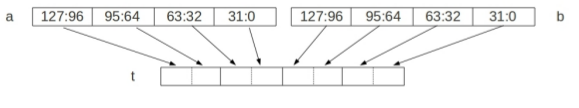
\includegraphics[width=130mm]{draw/horizontal.png}
\caption[Horizontal Operations in IDISA]{The logic of IDISA Horizontal Operations, cited from \cite{hua_idisa}.}
\label{figure:horizontal}
\end{figure}

\begin{figure}[ht!]
\centering
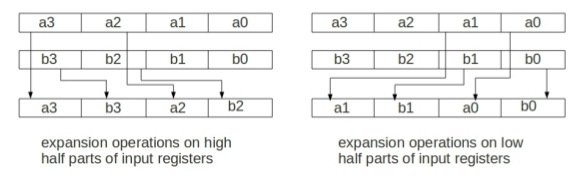
\includegraphics[width=130mm]{draw/expansion.png}
\caption[Expansion Operations in IDISA]{The logic of IDISA Expansion Operations, cited from \cite{hua_idisa}.}
\label{figure:expansion}
\end{figure}

The IDISA library divides SIMD operations into the following categories \cite{idisa_webpage}:
\begin{itemize}
    \item Vertical Operations (Template Class {\tt simd<w>}): They are the most common SIMD operations between two registers where {\tt w} is the field width. For example, {\tt simd<8>::add(A, B)} aligns registers A and B vertically and adds up the aligned 8-bit fields. Different fields are independent of each other.
    \item Horizontal Operations (Template Class {\tt hsimd<w>}): Operations like packing align the two operands horizontally, extract a portion of the bits in operands and concatenate into one full SIMD register. (Figure~\ref{figure:horizontal})
    \item Expansion Operations (Template Class {\tt esimd<w>}): Operations that double the width of fields like merging which takes the higher 64 bits of the two operands (A and B), concatenates the first field from A and the first field from B to get a new field with the width doubled. Do the same to the following fields until a full SIMD register C is generated. (Figure~\ref{figure:expansion})
    \item Field Movement Operations (Template Class {\tt mvmd<w>}): Operations that copy and move the entire fields. The content of these fields should not change.
    \item Full Register Operations (Template Class {\tt bitblock}): Operations that work with the contents of the whole SIMD registers. They are special vertical operations that has only one field.
\end{itemize}

The IDISA library claims to have better performance compared to the hand-written libraries. In the evaluation chapter, we will compare the performance of our LLVM back end with the IDISA library.

\subsection{Critical Parabix Operations}
There are at least five critical Parabix operations that can be the performance bottleneck and need special attention:
\begin{itemize}
    \item Transposition. This is the first step of every Parabix application and it can be the primary overhead of some Parabix application. There are two major algorithms: the ideal three-stage implementation and the byte-pack implementation. The byte-pack implementation utilizes packing on 16 bit field width which is widely available on commodity processors. The ideal three-stage implementation is less available but it is proved optimal in instruction count in the IDISA model. Details of these two algorithms can be found in \cite{inductive_doubling_principle}. We implement both of the algorithm with the modified LLVM and compare their performance in Chapter~\ref{six}.

    \item Inverse transposition. For some applications like the UTF-8 to UTF-16 transcoding, parallel bit streams need to be modified and translated back into byte streams, thus an inverse transposition is needed. As the inverse operation to the transposition, there are also two algorithms available which mirror the transposition algorithms. A detailed discussion can be found in \cite{rob_u8u16}.

    \item Long stream shift. Unbounded bit stream shift is translated into block-at-a-time shift. This operation shifts the whole SIMD register with the potential shift-in bits from the last block. We implement a peephole optimization in Chapter~\ref{five} that can improve the performance significantly.

    \item Long stream addition. The Pablo compiler deals with addition between unbounded bit streams using chained long stream additions, which adds two numbers as wide as the SIMD register with a carry-in bit and generates a carry-out bit. The naive approach chains 64-bit additions together to emulate 128-bit, 256-bit or 512-bit additions. Its time complexity grows linearly with the SIMD register size. A better algorithm is proposed in \cite{rob_regex} which could add up to 4096 bits wide integers in constant time. We implement the constant-time algorithm in Chapter~\ref{four}.

    \item Parallel deletion. This operation deletes bits from one bit stream at the positions identified by a deletion marker. Three different inductive doubling algorithms can be used for it. Refer to \cite{rob_u8u16} for further detail.
\end{itemize}

These operations take most of the run time in the application level profile, so a slight improvement could benefit the application greatly. We study the LLVM support of the first four operations in this work and leave the parallel deletion to be future work.

\section{LLVM Basics}
The \textit{Low Level Virtual Machine (LLVM)} is an open-source, well developed compiler tool that is dedicated to the compiler writers. It originates in 2000 with Lattner's Master thesis \cite{chris_msthesis} and has been gaining popularity ever since. Today it is developed into a high-performance static compiler back end with just-in-time compilers and life-long program analysis and optimization, which means program analysis and optimization in compile time, link time and run time \cite{llvm_ghc, llvm_cgo04}. It supports a variety of targets from Intel X86, PowerPC to the ARM mobile platform and hides the low-level target-specific issues for the compiler writers.

LLVM defines an intermediate representation (IR) as its virtual instruction set and IR is used as not only the input code to the LLVM tool chain but also the internal representation for analysis and optimization passes. This enables the programmer to use LLVM as a pipeline and to inspect output from each step. For example, with the C/C++ compiler of LLVM, Clang, source code in C/C++ is compiled into IR with different level of front end optimization. IR files are then linked together with link-time optimizations. The resulting IR is put through a good number of LLVM passes. LLVM optimizations are organized into passes. There are three types of passes \cite{llvm_pass}: analysis passes that collect information for other passes, transform passes that change the program and utility passes that provide general helper functionality for other passes. Each of the passes consumes LLVM IR as input and generates IR output. The improvements they make to the file can be easily checked by running these passes alone.

Although the IR is low-level, it preserves high-level static information through the strong type system and static single assignment (SSA) form. SSA form guarantees only one assignment to every variable. SSA helps calculate the high-level data flow \cite{cytron1991efficiently}. The main design goal of the IR is to be low-level enough so that most programming languages can target to it while maintaining the most high-level information to make aggressive back end optimization possible \cite{llvm_ghc}.

LLVM IR defines instructions and intrinsic functions. There are terminator instructions which produce control flow (return, branch, etc.), binary instructions (add, subtract, etc.), bitwise binary instructions (shift left/right, logic operations, etc.), memory instructions (load, store, etc.) and other instructions. Intrinsic functions are extension of IR instructions. Their names must all start with a "llvm." prefix \cite{llvm_lang_ref}. Example intrinsic functions are standard C library intrinsics (memcpy, sqrt, sin, floor, etc.), bit manipulation intrinsics (population count, byte swap, etc.), debugger intrinsics, exception handling intrinsics and so on. They can be general operations for all the platforms as well as target-specific; e.g.\ {\tt llvm.x86.sse2.psrli.w} corresponds to SSE2 native instruction $psrlw$. To achieve portability, we use none of these target-specific intrinsics in our work.

After optimization passes, the IR code is processed through the target-independent code generator and the machine code (MC) layer to become the native machine code. We describe the code generation process in detail in the next section as it is the major piece of logic we extend for parallel bit streams.

\section{LLVM Target-Independent Code Generator}
Although the name of the LLVM code generator contains ``target-independent'', it is not. There are genetic strategies that can be applied across different targets, but target specific information is heavily required throughout the code generation process. We want to clarify this point before we start to describe the LLVM code generator.

The first stage for code generation is Instruction Selection, which translates LLVM code into the target-specific machine instructions. After that, there are machine level optimizations like live-interval analysis and register allocation. Instruction Selection is done by the following steps \cite{llvm_code_gen} (we describe each step in the following text):

\begin{itemize}
  \item Initial SelectionDAG Construction: generate SelectionDAG from LLVM IR.
  \item DAG Combine 1
  \item Type Legalization Phase
  \item Post Type Legalization DAG Combine
  \item Operation Legalization Phase
  \item DAG Combine 2
  \item Instruction Select Phase
  \item Scheduling and Formation Phase
\end{itemize}

LLVM internally constructs a graph view of the input code called SelectionDAG where DAG is short for directed acyclic graph. Each node in the DAG represents an operation with an opcode, a number of operands and a number of return values. If the DAG node A uses the return value of another DAG node B, there will be an edge from B to A. The SelectionDAG enables a large variety of very-low-level optimization. And it also benefits the instruction scheduling process by recording the instruction dependency in the graph.

There are DAG combine passes after the initial construction and each legalization phase \cite{llvm_code_gen}, discussed shortly. DAG combine passes clean up SelectionDAG with both general and machine-dependent strategies, making the work easier for initial constructor and legalizers: they can focus on generating accurate SelectionDAG, good and legal operations with no worries of the messy output.

Instruction Select Phase is the bulk of target-specific logic that translates a legal SelectionDAG into a new DAG of target code with pattern matching facility. For example, a node of floating point addition followed by a floating point multiplication could be merged into one FMADDS node on the target that supports floating point multiply-and-add (FMA) operations \cite{llvm_code_gen}.

The Scheduling and Formation Phase assigns an order to each target instruction following the target's constraints. After that, a list of machine instructions are generated and the SelectionDAG is no longer needed.

Now we look at how LLVM deals with SIMD instructions. SIMD data are grouped into vectors and LLVM uses the notation \verb|<N x iX>| to represent a vector of N elements, where each of the element is an integer of X bits \cite{llvm_lang_ref, hybrid_simd_type_legalize}. \verb|<N x iX>| is also denoted as $vNiX$ as $vNiX$ is the internal type name used in the LLVM source code; e.g.\ \verb|<4 x i32>| is the same with $v4i32$. Various operations can be applied on vectors and the LLVM back end knows how to lower them into proper machine instructions.

In LLVM IR, programmers can write any kind of vectors, even $v1024i3$. Those vectors may not be supported by the target machine. LLVM has the notion of "legal" vs. "illegal" types. Legality is a target-specific concept. A DAG node is legal if it only uses the supported operation on the supported types. Unsupported types are illegal types for the target. For example, $i1$ is not supported in X86, it is illegal together with all the operations that take $i1$ operands or return $i1$ values. Addition on $v16i8$ is legal for X86 SSE2 but multiplication on $v16i8$ is not since there is no native support of it. The type $v16i8$ is considered to be legal in this case. LLVM code generator has all the target details. It uses type legalization and operation legalization phases to turn illegal type or DAG into legal\cite{llvm_code_gen}.

Type legalization phase has three ways to legalize vector types\cite{hybrid_simd_type_legalize}: \textit{Scalarization}, \textit{Vector Widening} and \textit{Vector Element Promotion}.

\begin{itemize}
    \item \textbf{Scalarization} splits the vector into multiple scalars. It is often used for the transformation from $v1iX$ to $iX$.
    \item \textbf{Vector Widening} adds dummy elements to make the vector fit the right register size. It does not change the type of the elements, e.g.\ $v4i8$ to $v16i8$.
    \item \textbf{Vector Element Promotion} preserves the number of elements, but promotes the element type to a wider size, e.g.\ $v4i8$ to $v4i32$.
\end{itemize}

After type legalization, we may still have an illegal DAG node. This is because some operation on the legal type is not supported by the target. We need the operation legalization phase. There are three strategies in this phase:

\begin{itemize}
    \item \textbf{Expansion}: Use another sequence of operations to emulate the operation. Expansion strategy is often general in the sense that it may use slow operations such as memory load and store, but it generates native code with correct outcomes.
    \item \textbf{Promotion}: Promote the operand type to a larger type that the operation supports.
    \item \textbf{Custom}: Write target-specific code to implement the legalization. This is similar to Expansion, but with a specific target in mind.
\end{itemize}

No illegal type should be introduced in the operation legalization phase which puts a limitation on the machine-independent legalize strategies: $i8$ is the minimum integer type on X86 and programmer needs to extend every integer less than 8 bits to $i8$ before returning it to the DAG\@. On the other hand DAG combine is different, you can choose the combine timing on your own. If you choose to combine before type legalization phase, you can freely introduce illegal types into your combined results.

The current legalization mechanism of LLVM is not sufficient to handle Parabix code efficiently. We propose new strategies and redefine legality in Chapter~\ref{four}.

\section{Summary}
In this chapter we reviewed the Parabix technology which is a parallel text processing model and IDISA library which is a C++ library for SIMD programming. We also provided LLVM basics and described its target-independent code generator. The IDISA library has to maintain target-specific header files and is hard to further optimize outside the function scope. So we propose to replace the IDISA library with a LLVM back end in the next chapter.
